%---------------------------------- Optimization frame -------------------------------
\begin{frame}{Global HPO workflow}
            \begin{figure}
                \centering
                \begin{tikzpicture}[node distance=2cm]

% Define block styles
\tikzstyle{startstop} = [rectangle, rounded corners, minimum width=3cm, minimum height=1cm,text centered, draw=black, fill=green!30]
\tikzstyle{io} = [trapezium, trapezium left angle=70, trapezium right angle=110, minimum width=3cm, minimum height=1cm, text centered, draw=black, fill=blue!30]
\tikzstyle{process} = [rectangle, minimum width=3cm, minimum height=1cm, text centered, draw=black, fill=blue!20]
\tikzstyle{decision} = [diamond, minimum width=3cm, minimum height=1cm, text centered, draw=black, fill=red!30]
\tikzstyle{arrow} = [thick,->,>=stealth]

% Nodes
\node (start) [startstop] {Training Data};
\node (preprocess) [process, below of=start] {Preprocessing};
\node (stop) [decision, below of=preprocess] {Stop?};
\node (hpo) [process, right of=stop, xshift=3cm] {Hyperparameter Optimization (HPO)};
\node (finalmodel) [startstop, below of=stop] {Final Model};
\node (validation) [startstop, above of=hpo] {Validation Data};

% Arrows
\draw [arrow] (start) -- (preprocess);
\draw [arrow] (preprocess) -- (stop);
\draw [arrow] (stop) -- node[anchor=south] {No} (preprocess);
\draw [arrow] (stop) -- node[anchor=south] {Yes} (finalmodel);
\draw [arrow] (finalmodel) -- (hpo);
\draw [arrow] (validation) -- (hpo);
\draw [arrow] (hpo) -- (finalmodel);
\end{tikzpicture}
                \caption{HPO workflow}
            \end{figure}
    
\end{frame}

%---------------------------------- Optimization -------------------------------
\begin{frame}[allowframebreaks]{Optimization : generate the new solution}
    \begin{block}{Frameworks}
        BoTorch for all gaussian processes, everything in python.
    \end{block}

    \framebreak

    \begin{columns}
        \begin{column}{0.3\textwidth}
            \textbf{Partition Based Algorithm : Simultaneous Optimistic Optimization (SOO)}

            Perform a K-inary partition of the space, evaluating every center of partition during the expansion of a node.
            
        \end{column}        
        \begin{column}{0.7\textwidth}
            \begin{figure}[h]
                \centering
                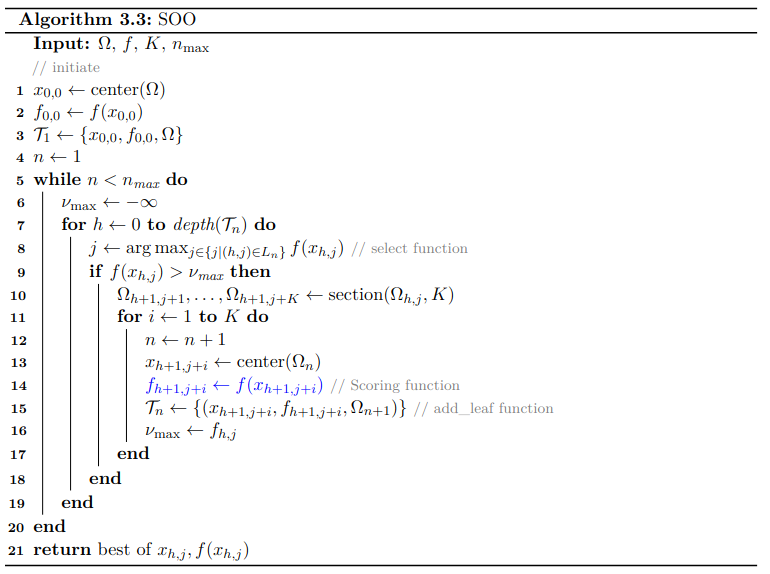
\includegraphics[height = 6cm]{imgs/algo/soo.png}
            \end{figure}
        \end{column}
    \end{columns}

    \framebreak

    \begin{columns}
        \begin{column}{0.3\textwidth}
            \textbf{Surrogate Model Based Optimization : Bayesian Optimization with Gaussian Process (BO-GP)}

            Use Gaussian Process as a surrogate for the objective function, and optimize it to found the most promising point to evaluate
            
        \end{column}        
        \begin{column}{0.7\textwidth}
            \begin{figure}[h]
                \centering
                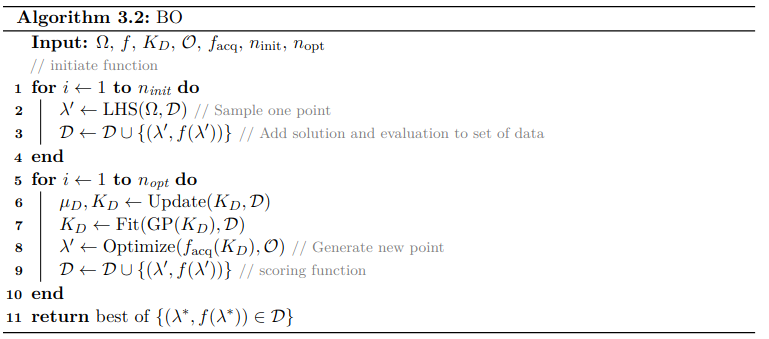
\includegraphics[height = 6cm]{imgs/algo/bo.png}
            \end{figure}
        \end{column}
    \end{columns}

    \framebreak

    \begin{columns}
        \begin{column}{0.5\textwidth}
            \textbf{Hybridation : Bayesian Multi-Scale Optimistic Optimization(BaMSOO)}

            Replace the scoring of SOO with a BO-GP based approximation to determine if it's relevant to evaluate the point.
            \begin{equation}
                \begin{split}
                \mathcal{UCB}(x| \mathcal D_t) = \mu(x|\mathcal D_t) +  B_N * \sigma(x|\mathcal D_t) 
                \\ \text{with } B_N = \sqrt{2 \log (\pi^2 N^2/6 \eta)} , \eta \in (0,1)      
                \end{split}  
                \label{eq:ucb}
            \end{equation}
            
        \end{column}        
        \begin{column}{0.5\textwidth}
            \begin{figure}[h]
                \centering
                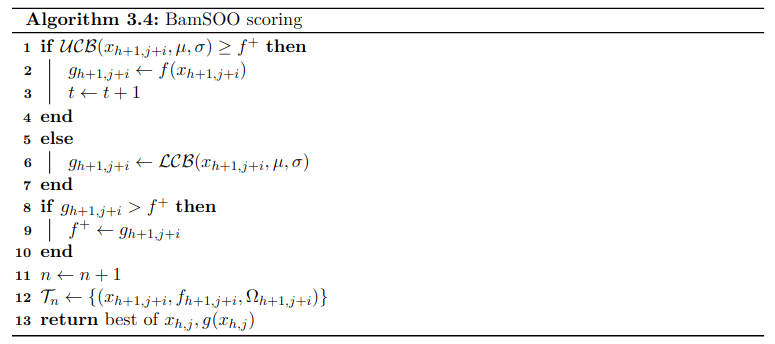
\includegraphics[height = 5cm]{imgs/algo/bamsoo_score.png}
            \end{figure}
        \end{column}
    \end{columns}

        
\end{frame}



%---------------------------------- Evaluation Function -------------------------------
\begin{frame}{Evaluate the solution}
    Use LitGPT framework with it's CLI to perform an evaluation of a solution. All models and datasets are taken from HuggingFace Hub.
    \begin{block}{Training}
        \begin{itemize}
            \item Model : Llama-3.2-3B
            \item dataset : Alpaca
            \item 1 epochs of training
            \item Fully Sharded Data Parallelism (FSDP) as distributed strategy
        \end{itemize}
    \end{block}

    \begin{block}{Evaluating}
        Based on lm\_eval library
        \begin{itemize}
            \item validation dataset : Hellaswag
            \item testing dataset : MMLU
        \end{itemize}
    \end{block}

    
\end{frame}